\documentclass[aspectratio=169,10pt]{beamer}

\usetheme{metropolis}
\usepackage{appendixnumberbeamer}
\usepackage{booktabs}
\usepackage{amsmath,amssymb}
\usepackage{graphicx}
\usepackage[table]{xcolor}
\usepackage{tikz}
\usepackage{pgfplots}
\pgfplotsset{compat=1.18}
\usepackage{caption}
\captionsetup[figure]{font=scriptsize,labelfont=scriptsize}

\graphicspath{{../visualizations/}{../results/}}

% Colors
\definecolor{cfmblue}{RGB}{41,98,255}
\definecolor{ddpmred}{RGB}{211,47,47}
\definecolor{accentgreen}{RGB}{46,125,50}

\setbeamercolor{frametitle}{bg=cfmblue!90!black,fg=white}
\setbeamercolor{progress bar}{fg=cfmblue}
\setbeamercolor{alerted text}{fg=ddpmred}

\title{Conditional flow matching vs.\ diffusion models}
\subtitle{A systematic comparison on CIFAR-10}
\author{Ali Dor \and Elora Drouilhet}
\institute{CentraleSup\'elec/MVA --- Advanced Deep Learning course}
\date{March 23, 2026}

\begin{document}

% ============================================================
\begin{frame}[plain]
\maketitle
\end{frame}

% ============================================================
\begin{frame}{Outline}
\tableofcontents
\end{frame}

% ============================================================
\section{Motivation}

\begin{frame}{Why flow matching?}
\begin{columns}[T]
\begin{column}{0.55\textwidth}
\textbf{The problem with diffusion models:}
\begin{itemize}
    \item DDPM needs \alert{many steps} to generate one image
    \item DDIM reduces steps but quality \alert{saturates at a certain point}
    \item Curved denoising paths are hard to integrate
\end{itemize}

\vspace{1em}
\textbf{Flow matching promise:}
\begin{itemize}
    \item Learn \textcolor{cfmblue}{\textbf{straight}} transport paths from noise to data
    \item ODE-based: use any solver, any \# steps
    \item OT coupling $\Rightarrow$ nearly linear trajectories
    \item \textcolor{accentgreen}{\textbf{Same quality, fewer steps}}
\end{itemize}
\end{column}
\begin{column}{0.42\textwidth}
\centering

\includegraphics[width=\textwidth]{coupling_comparison.png}\\[0.5em]
{\scriptsize Independent vs.\ OT coupling on 2D data}
\end{column}
\end{columns}
\end{frame}

% ============================================================
\section{Background}

\begin{frame}{DDPM \& DDIM}
\begin{columns}[T]
\begin{column}{0.55\textwidth}
\textbf{DDPM} --- Denoising Diffusion Probabilistic Model:
\begin{itemize}
    \item Gradually adds Gaussian noise to data over $T{=}1000$ steps
    \item Trains a network $\epsilon_\theta$ to predict the added noise:
$$\mathcal{L}_{\text{DDPM}} = \mathbb{E}_{t,\mathbf{x}_0,\epsilon}\left[\|\epsilon - \epsilon_\theta(\mathbf{x}_t, t)\|^2\right]$$
    \item Generates by iteratively denoising $\mathbf{x}_T \to \mathbf{x}_0$
    \item Slow: requires all 1000 steps
\end{itemize}

\vspace{0.5em}
\textbf{DDIM} --- deterministic shortcut:
\begin{itemize}
    \item Reuses the same trained DDPM model
    \item Skips timesteps: 10--100 steps instead of 1000
    \item But: approximation errors accumulate, quality saturates
\end{itemize}
\end{column}
\begin{column}{0.42\textwidth}
\centering
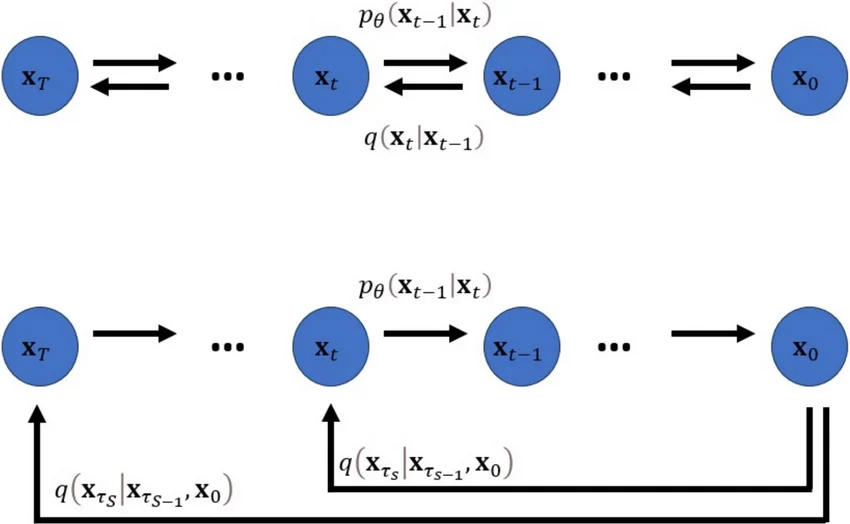
\includegraphics[width=\textwidth]{DDPMvsDDIM.jpg}\\[0.3em]
{\scriptsize The forward and reverse processes of DDPM (top) and DDIM (bottom)}
\end{column}
\end{columns}
\end{frame}

\begin{frame}{Flow matching: a different paradigm}
\begin{columns}[T]
\begin{column}{0.55\textwidth}
\textbf{Key idea}: learn a velocity field, not noise

\textbf{OT interpolation path}:
$$\mathbf{x}_t = (1{-}t)\,\mathbf{x}_0 + t\,\mathbf{x}_1$$
$$\mathbf{u}_t = \mathbf{x}_1 - \mathbf{x}_0 \quad \text{(constant velocity!)}$$

\textbf{Training} (predict velocity):
$$\mathcal{L}_{\text{CFM}} = \mathbb{E}_{t,\mathbf{x}_0,\mathbf{x}_1}\left[\|v_\theta(\mathbf{x}_t, t) - \mathbf{u}_t\|^2\right]$$

\textbf{Sampling}: solve ODE from $t{=}0 \to 1$
$$\frac{d\mathbf{x}}{dt} = v_\theta(\mathbf{x}_t, t)$$

\begin{itemize}
    \item \textcolor{cfmblue}{\textbf{Straight paths}} $\Rightarrow$ easy to integrate
    \item Any ODE solver, any number of steps
\end{itemize}
\end{column}
\begin{column}{0.42\textwidth}
\centering

\includegraphics[width=\textwidth]{vector_fields_2d.png}\\[0.3em]
{\scriptsize Learned velocity fields at different $t$}
\end{column}
\end{columns}
\end{frame}

\begin{frame}{ODE solvers for flow matching}
\centering
\vspace{0.5em}
{\small \textbf{Table: ODE solvers compared}}\\[0.5em]
\begin{tabular}{lccc}
\toprule
\textbf{Solver} & \textbf{Order} & \textbf{NFE/step} & \textbf{Best for} \\
\midrule
Euler & 1st & 1 & Simplest baseline \\
Midpoint & 2nd & 2 & Low NFE (10--50) \\
RK4 & 4th & 4 & High NFE (100+) \\
\bottomrule
\end{tabular}

\vspace{1.5em}
\textbf{Key insight}: at fixed NFE budget, higher-order solvers take fewer but more accurate steps.
\end{frame}

% ============================================================
\section{Our implementation}

\begin{frame}{Architecture}
\begin{columns}[T]
\begin{column}{0.48\textwidth}
\textbf{UNet} (DDPM/DDIM \& unconditional CFM):
\begin{itemize}
    \item 128 base channels
    \item Channel mult: $[1, 2, 2, 2]$
    \item 4 attention heads, GroupNorm-32
    \item Sinusoidal time embeddings
    \item Adam, lr $= 2 \times 10^{-4}$
    \item 500 epochs, EMA 0.9999
\end{itemize}

\vspace{0.5em}
\textbf{Evaluation protocol}:
\begin{itemize}
    \item 10,000 generated samples
    \item FID and Inception Score
    \item NFE sweep: 10, 20, 50, 100
    \item Google Colab (T4 / A100)
\end{itemize}
\end{column}
\begin{column}{0.48\textwidth}
\textbf{SimpleFlowUNet} (class-conditional CFM):
\begin{itemize}
    \item 128 base channels
    \item Channel mult: $[1, 2, 4]$
    \item Single-head attention, GroupNorm-8
    \item Learned class embeddings (10 classes)
    \item 10\% class dropout $\Rightarrow$ CFG
    \item AdamW, lr $= 2 \times 10^{-4}$
    \item 210 epochs, EMA 0.999
\end{itemize}
\end{column}
\end{columns}
\end{frame}

\begin{frame}{Architecture}
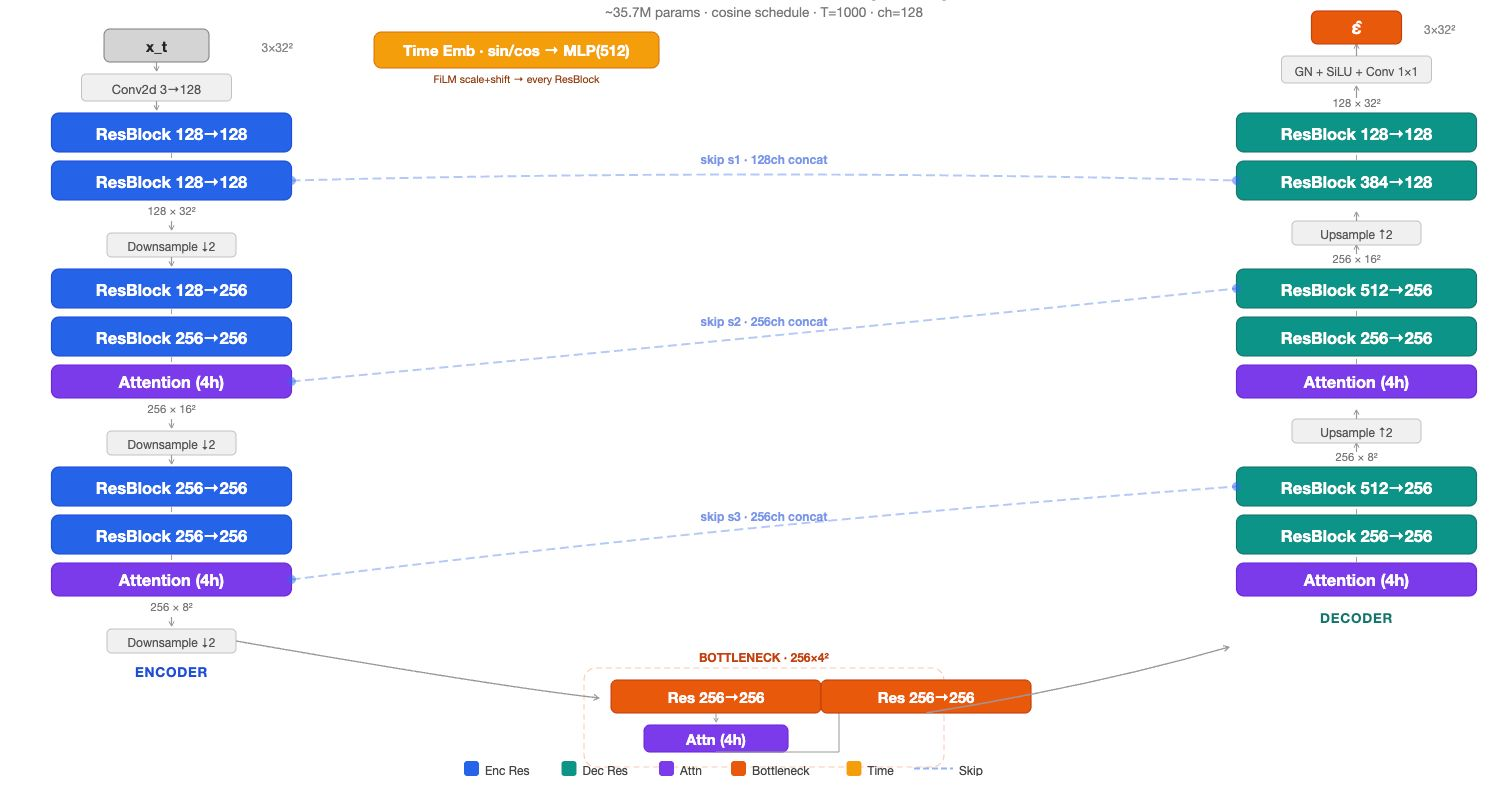
\includegraphics[width=\textwidth]{Arch.jpeg}\\[0.3em]
\end{frame}


% ============================================================
\section{2D toy experiments}

\begin{frame}{Learning to transport: 2D visualization}
\begin{columns}[c]
\begin{column}{0.48\textwidth}
\centering

\includegraphics[width=\textwidth]{vector_fields_2d.png}\\[0.3em]
{\scriptsize Velocity fields at $t=0.0, 0.25, 0.5, 0.75, 1.0$}
\end{column}
\begin{column}{0.48\textwidth}
\centering

\includegraphics[width=\textwidth]{toy_2d_samples.png}\\[0.3em]
{\scriptsize Generated 2D samples vs.\ target distribution}
\end{column}
\end{columns}

\vspace{0.5em}
The model learns time-varying velocity fields that smoothly transport Gaussian noise to complex multi-modal distributions.
\end{frame}

\begin{frame}{Why optimal transport matters}
\centering

\includegraphics[width=0.75\textwidth]{coupling_comparison.png}

\vspace{0.5em}
\begin{columns}[T]
\begin{column}{0.48\textwidth}
\centering
\textbf{Independent coupling}\\
Paths cross $\Rightarrow$ curved trajectories\\
Harder for ODE solvers
\end{column}
\begin{column}{0.48\textwidth}
\centering
\textbf{\textcolor{cfmblue}{OT coupling}}\\
Non-crossing, straight paths\\
Easy to integrate accurately
\end{column}
\end{columns}
\end{frame}

% ============================================================
\section{CIFAR-10 results}

\begin{frame}{Main results: FID vs NFE}
\begin{columns}[T]
\begin{column}{0.55\textwidth}
\centering
{\small \textbf{Table: Full comparison on CIFAR-10}}\\[0.3em]
\scriptsize
\begin{tabular}{@{}llrr@{}}
\toprule
\textbf{Method} & \textbf{Solver} & \textbf{NFE} & \textbf{FID}\,$\downarrow$ \\
\midrule
DDPM & --- & 1000 & 13.06 \\
\midrule
DDIM & --- & 10 & 22.18 \\
DDIM & --- & 20 & 18.95 \\
DDIM & --- & 50 & 17.96 \\
DDIM & --- & 100 & \alert{18.43\,$\uparrow$} \\
\midrule
OT-CFM & Midpoint & 10 & 17.53 \\
OT-CFM & Midpoint & 20 & 14.80 \\
OT-CFM & Midpoint & 50 & 12.02 \\
OT-CFM & Midpoint & 100 & 11.21 \\
OT-CFM & RK4 & 100 & {\color{green}\textbf{10.65}} \\
\midrule
Cond.\ CFM & Midpoint & 50 & 13.17 \\
Cond.\ CFM & RK4 & 100 & 12.19 \\
\bottomrule
\end{tabular}
\end{column}
\begin{column}{0.42\textwidth}
\textbf{Key findings:}

\vspace{0.5em}
\textbf{Best FID: 10.65}\\
(OT-CFM, RK4, 100 NFE)

\vspace{0.5em}
vs.\ DDPM: 13.06 at 1000 NFE\\
$\Rightarrow$ \textbf{20$\times$ speedup}

\vspace{0.5em}
\alert{DDIM degrades} past 50 NFE\\
(18.43 at 100 vs.\ 17.96 at 50)

\vspace{0.5em}
OT-CFM at \textbf{20 NFE} (14.80)\\
already beats best DDIM (17.96)
\end{column}
\end{columns}
\end{frame}

\begin{frame}{Best results summary}
\centering
{\small \textbf{Table: Best FID per model family}}\\[0.5em]
\large
\begin{tabular}{@{}lrrll@{}}
\toprule
\textbf{Model} & \textbf{Best FID} & \textbf{NFE} & \textbf{Solver} & \textbf{ms/img} \\
\midrule
DDPM & 13.06 & 1000 & --- & 205.0 \\
DDIM & 17.96 & 50 & --- & 10.5 \\
\rowcolor{cfmblue!10}
\textbf{OT-CFM} & \textbf{10.65} & \textbf{100} & \textbf{RK4} & \textbf{20.7} \\
Cond.\ CFM & 12.19 & 100 & RK4 & 24.3 \\
\bottomrule
\end{tabular}

\vspace{1.5em}
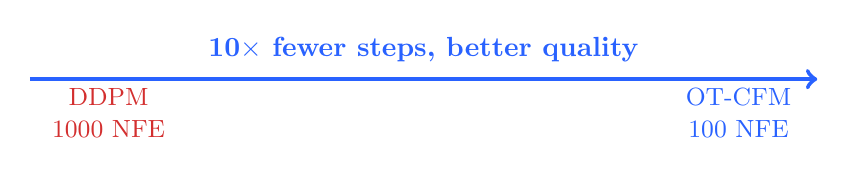
\begin{tikzpicture}
\draw[cfmblue,ultra thick,->] (0,0) -- (10,0);
\node[above,cfmblue] at (5,0.1) {\textbf{10$\times$ fewer steps, better quality}};
\node[below,ddpmred] at (1,0) {\small DDPM};
\node[below,ddpmred] at (1,-0.4) {\small 1000 NFE};
\node[below,cfmblue] at (9,0) {\small OT-CFM};
\node[below,cfmblue] at (9,-0.4) {\small 100 NFE};
\end{tikzpicture}
\end{frame}

\begin{frame}{Generation quality: samples}
\begin{columns}[c]
\begin{column}{0.48\textwidth}
\centering
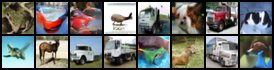
\includegraphics[width=0.95\textwidth]{epoch_0500_cfm.png}\\[0.3em]
{\scriptsize OT-CFM unconditional samples (epoch 500)}
\end{column}
\begin{column}{0.48\textwidth}
\centering
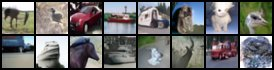
\includegraphics[width=0.95\textwidth]{epoch_0500_ddpm.png}\\[0.3em]
{\scriptsize DDPM samples (epoch 500)}
\end{column}
\end{columns}
\end{frame}

\begin{frame}{Latent interpolation}
\begin{columns}[T]
\begin{column}{0.48\textwidth}
\centering

\includegraphics[width=\textwidth]{interpolation_cfm.png}\\[0.3em]
{\scriptsize OT-CFM interpolation}
\end{column}
\begin{column}{0.48\textwidth}
\centering

\includegraphics[width=\textwidth]{interpolation_ddim.png}\\[0.3em]
{\scriptsize DDIM interpolation}
\end{column}
\end{columns}

\vspace{0.5em}
Both models support smooth latent interpolation, but CFM transitions are notably smoother due to the straight OT paths.
\end{frame}

\begin{frame}{Class-conditional generation with CFG}
\centering

\includegraphics[width=0.8\textwidth]{conditional_cfg_comparison.png}\\
{\scriptsize Effect of classifier-free guidance on class-conditional generation}

\vspace{-1em}
\[
v = v_{\text{uncond}} + s\,(v_{\text{cond}} - v_{\text{uncond}})
\]
\end{frame}


% ============================================================
\section{ODE inversion \& image editing}

\begin{frame}{ODE inversion: the key idea}
\begin{columns}[T]
\begin{column}{0.55\textwidth}
CFM's ODE is \textbf{deterministic and invertible}:

\vspace{0.5em}
\textbf{Forward} (generation):
$$z_0 \xrightarrow{t=0 \to 1} x_1$$

\textbf{Backward} (inversion):
$$x_1 \xrightarrow{t=1 \to 0} z_0$$

\vspace{0.5em}
Every real image has a unique ``address'' in noise space.

\vspace{0.5em}
\textbf{This enables:}
\begin{itemize}
    \item Encode any real image to noise
    \item Edit by manipulating the noise
    \item Decode back to get edited image
\end{itemize}

\vspace{0.5em}
\alert{DDPM cannot do this} --- its sampling is stochastic.
\end{column}
\begin{column}{0.42\textwidth}
\centering
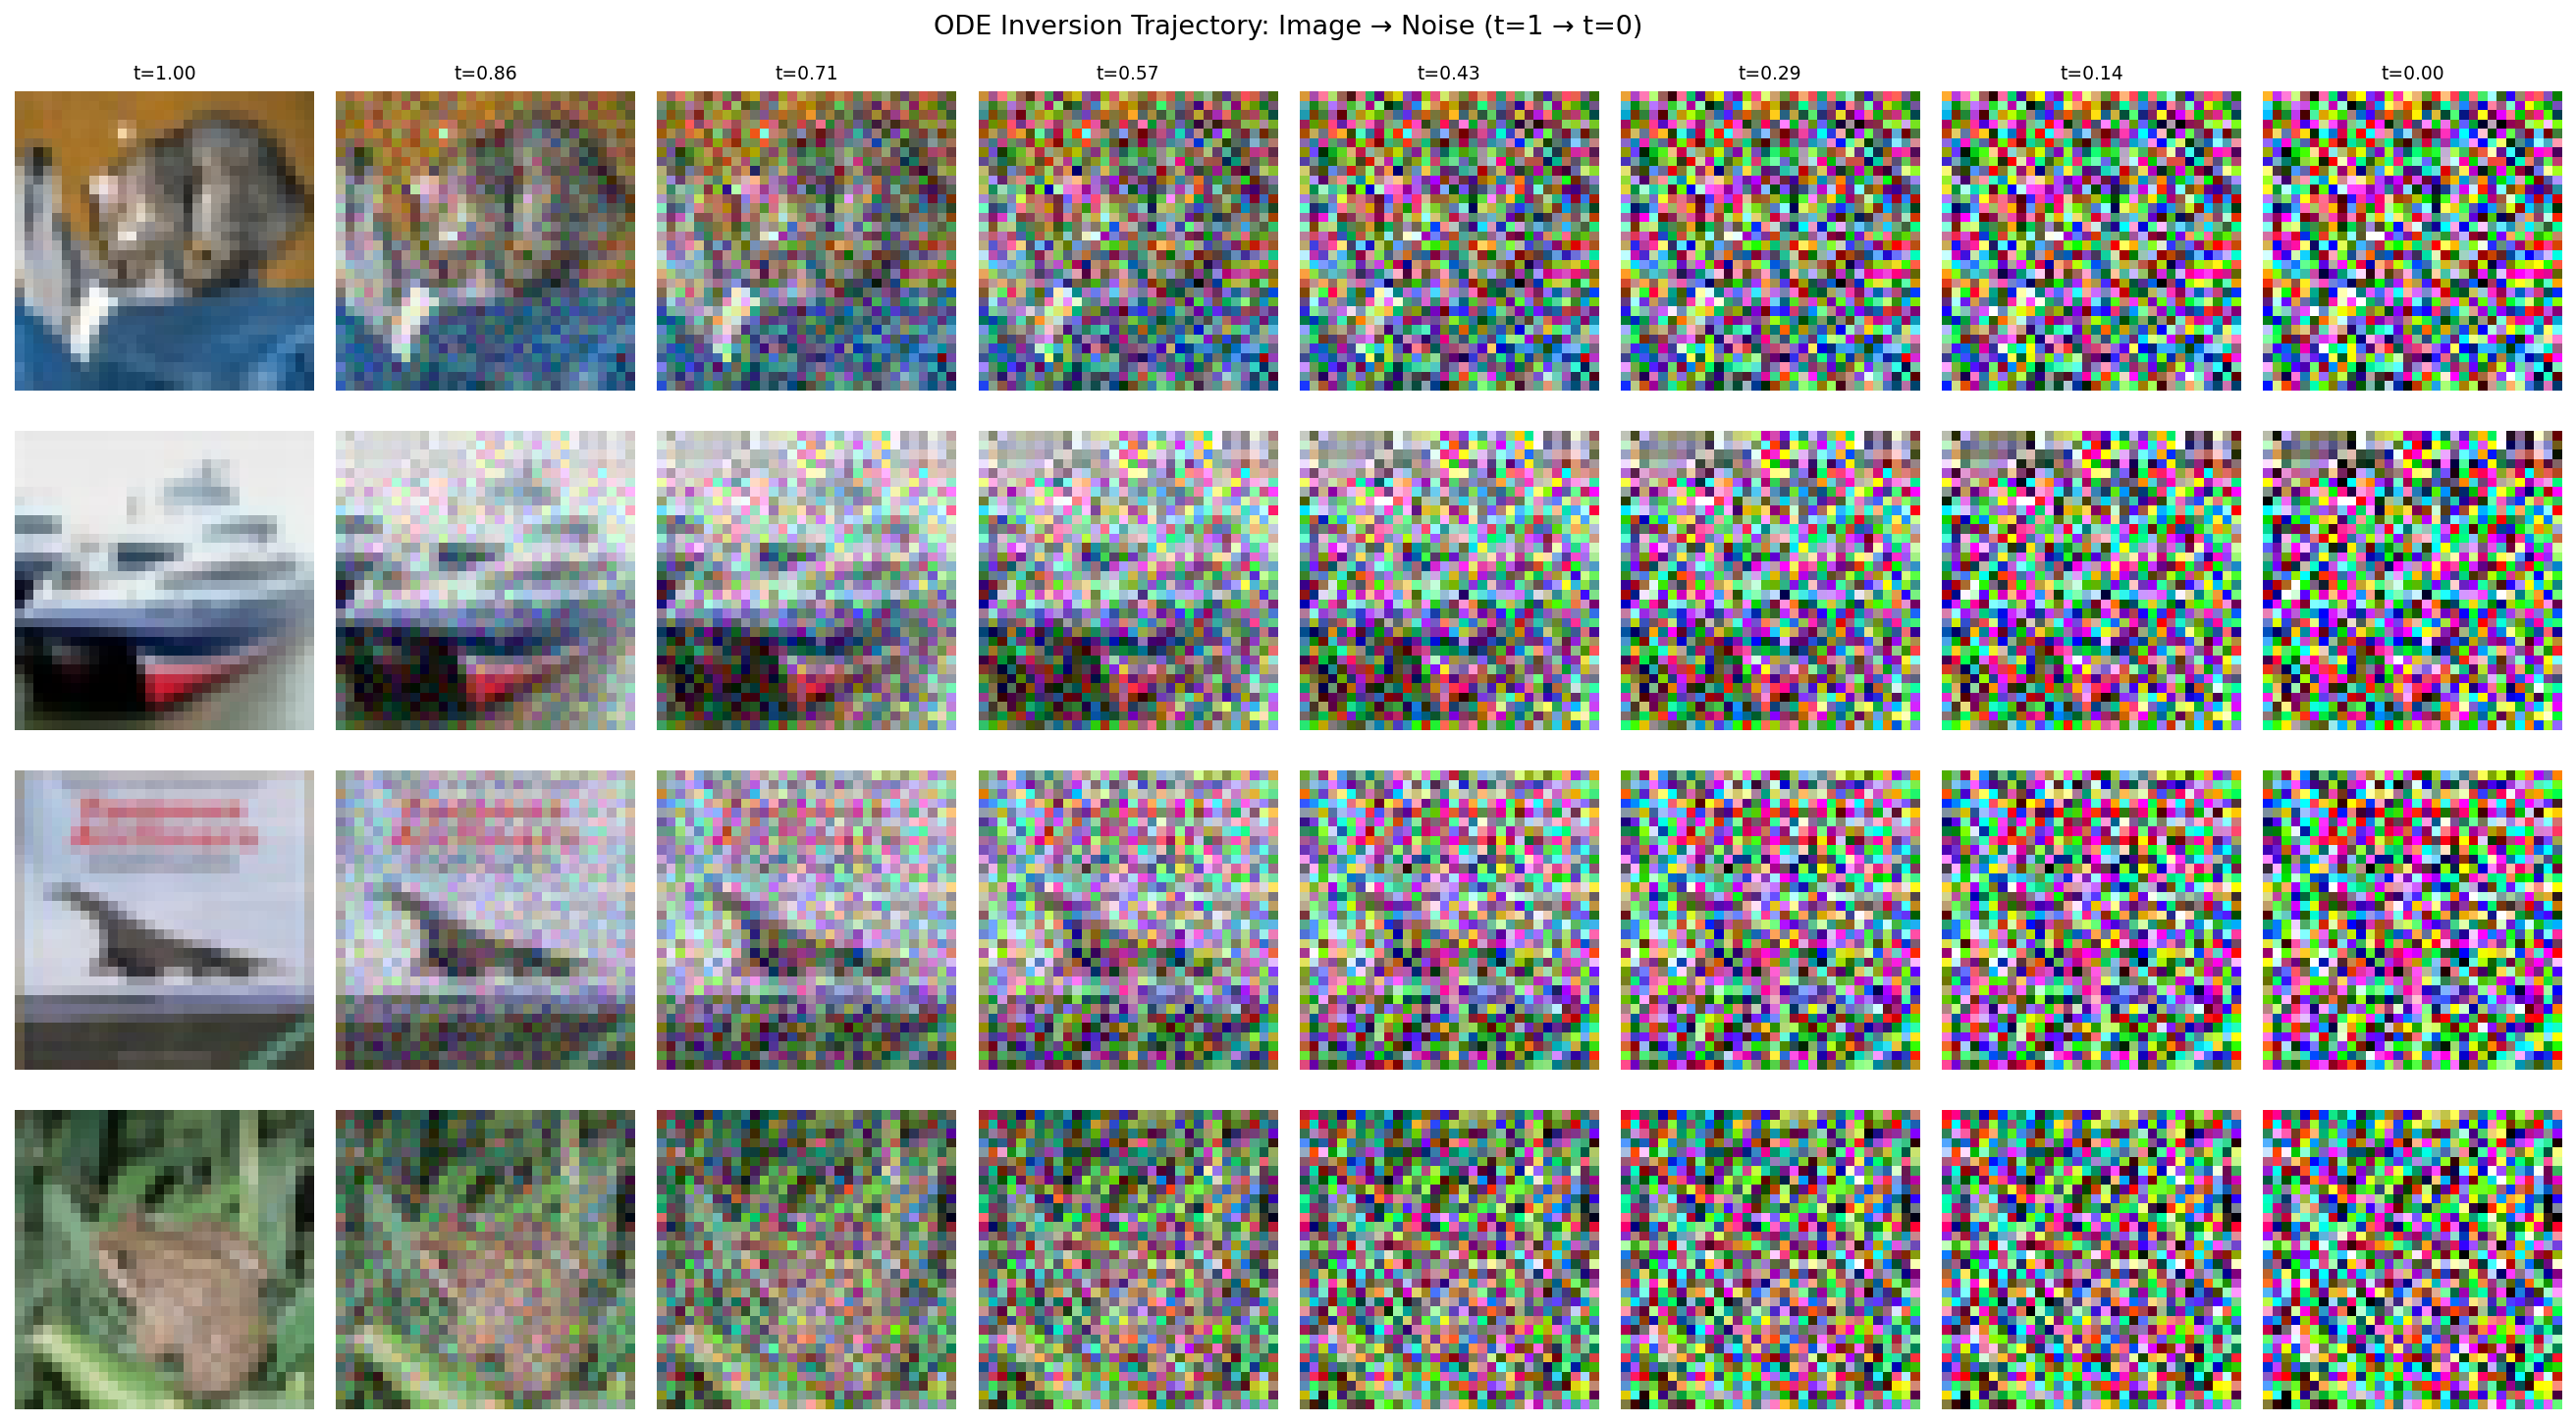
\includegraphics[width=\textwidth]{inversion_trajectory.png}\\[0.3em]
{\scriptsize Real images dissolving into noise (t=1$\to$0)}
\end{column}
\end{columns}
\end{frame}

\begin{frame}{Reconstruction: encode $\to$ decode}
\centering
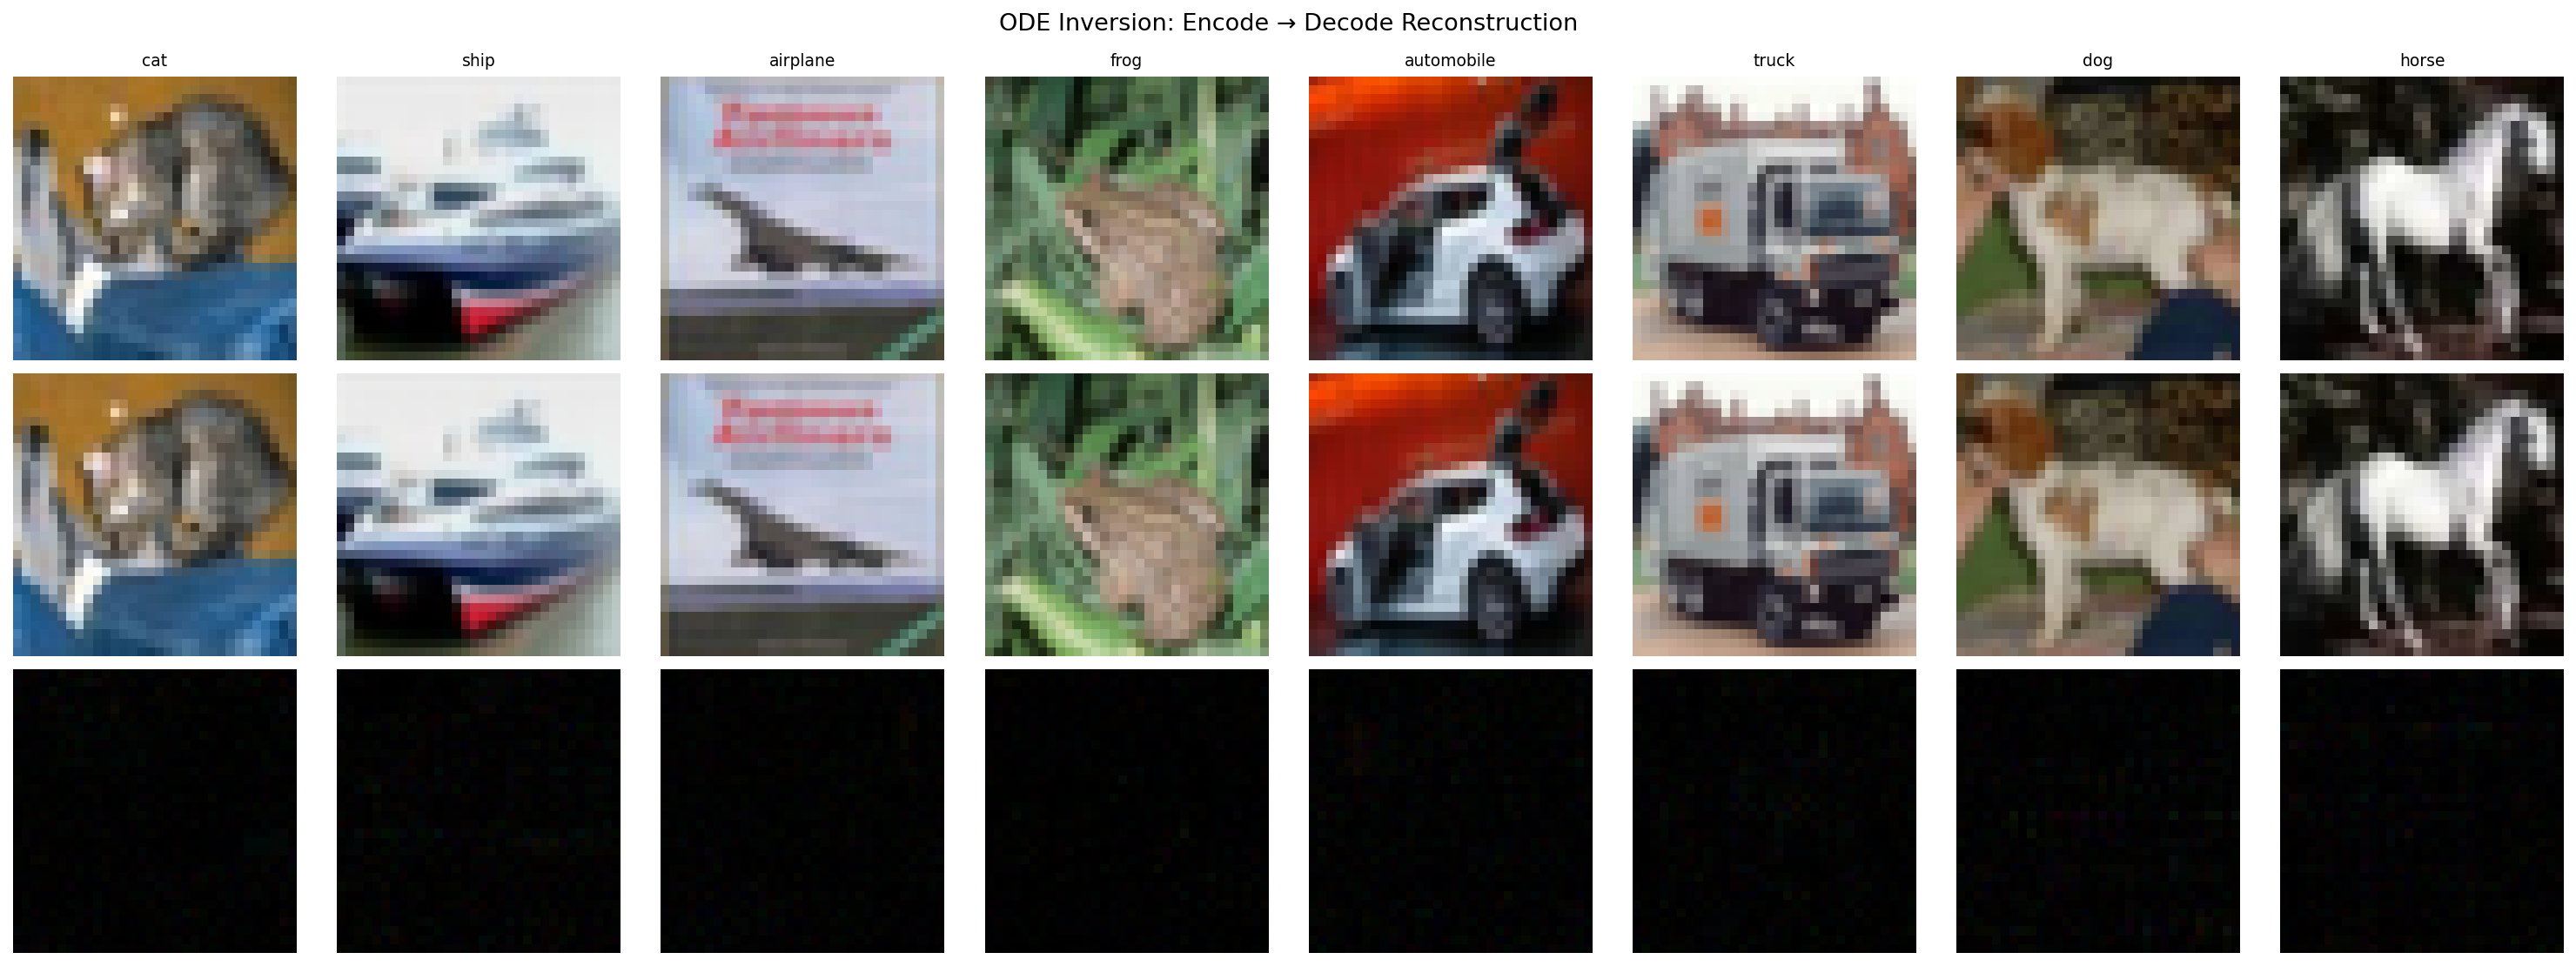
\includegraphics[width=0.85\textwidth]{reconstruction.png}

\vspace{0.5em}
\begin{itemize}
    \item Top: original CIFAR-10 images (one per class)
    \item Middle: reconstructed via backward ODE $\to$ forward ODE
    \item Bottom: pixel difference (5$\times$ amplified) --- \textcolor{accentgreen}{\textbf{near-zero}}
\end{itemize}

\vspace{0.3em}
The ODE inversion is \textbf{near-perfect}, confirming the model learned an accurate invertible flow.
\end{frame}

\begin{frame}{Latent perturbations \& attribute editing}
\begin{columns}[T]
\begin{column}{0.48\textwidth}
\centering
{\small \textbf{Latent perturbations}}\\[0.3em]
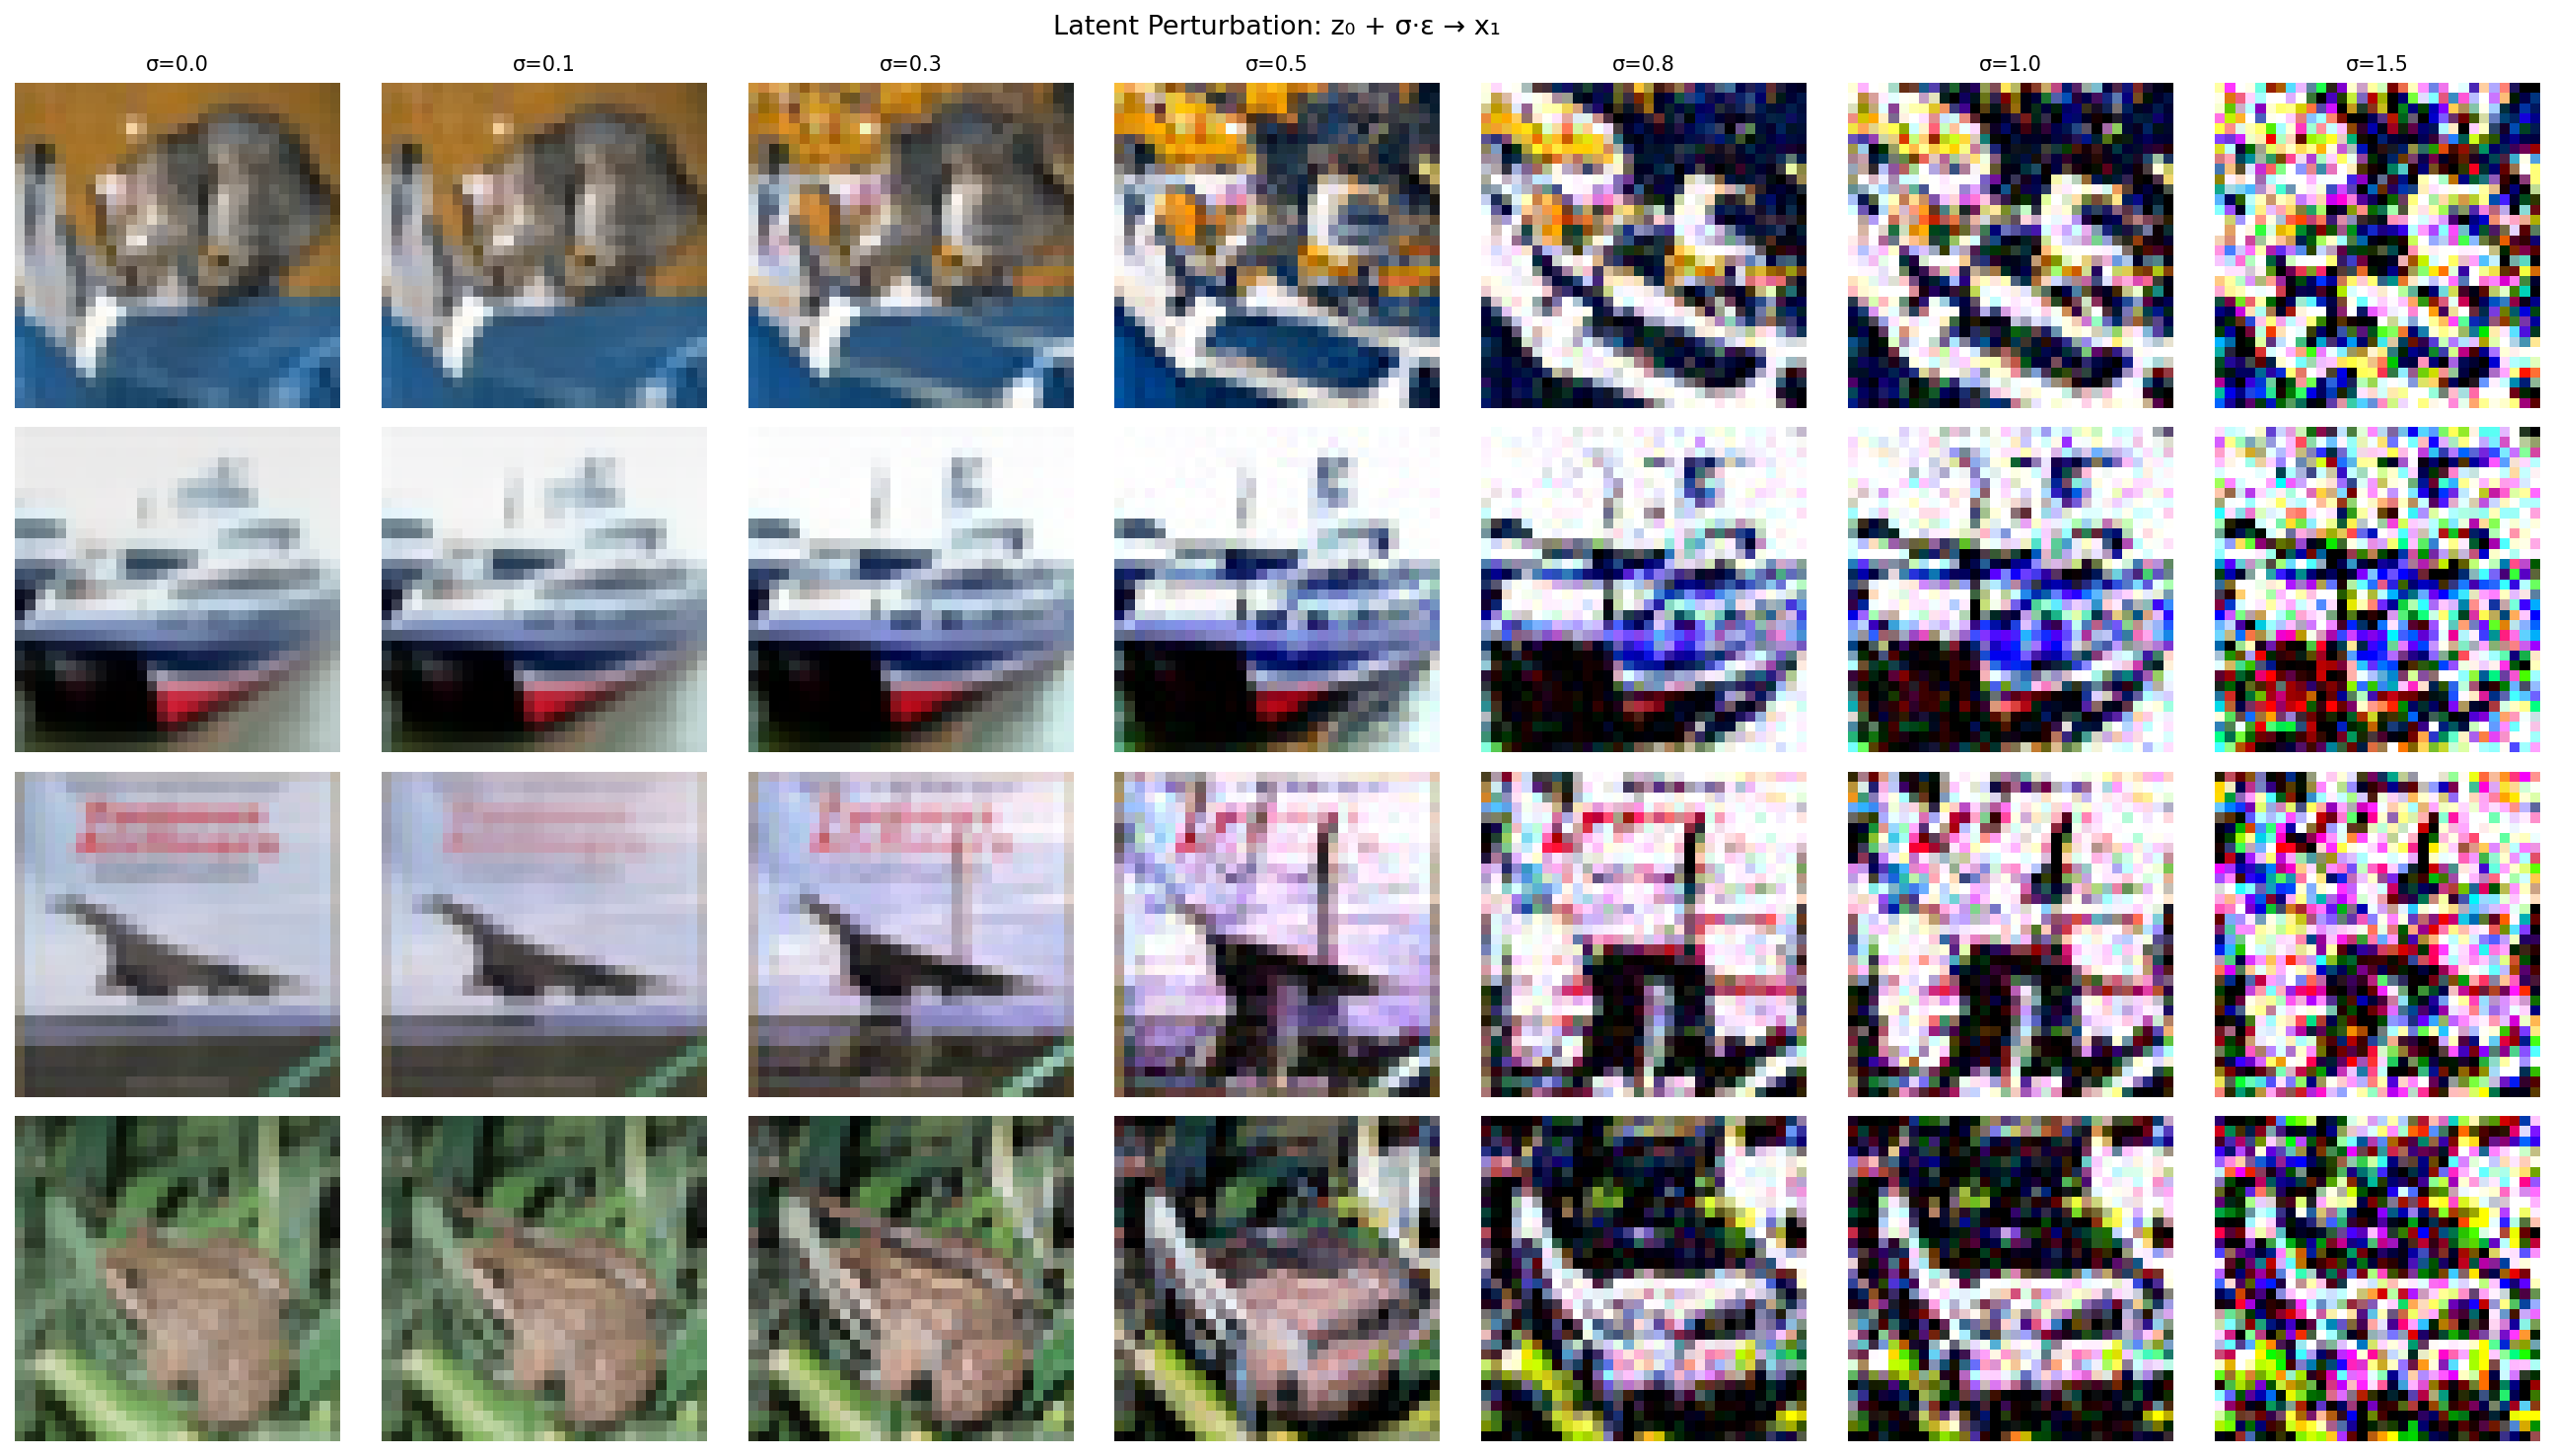
\includegraphics[width=\textwidth]{perturbations.png}\\[0.3em]
{\scriptsize Perturb $z_0 + \sigma\epsilon$, then decode.\\
$\sigma{=}0$: original. $\sigma{=}0.3$: subtle change.\\
$\sigma{=}1.5$: content destroyed.\\
Latent space is smooth and locally stable.}
\end{column}
\begin{column}{0.48\textwidth}
\centering
{\small \textbf{Attribute editing}}\\[0.3em]
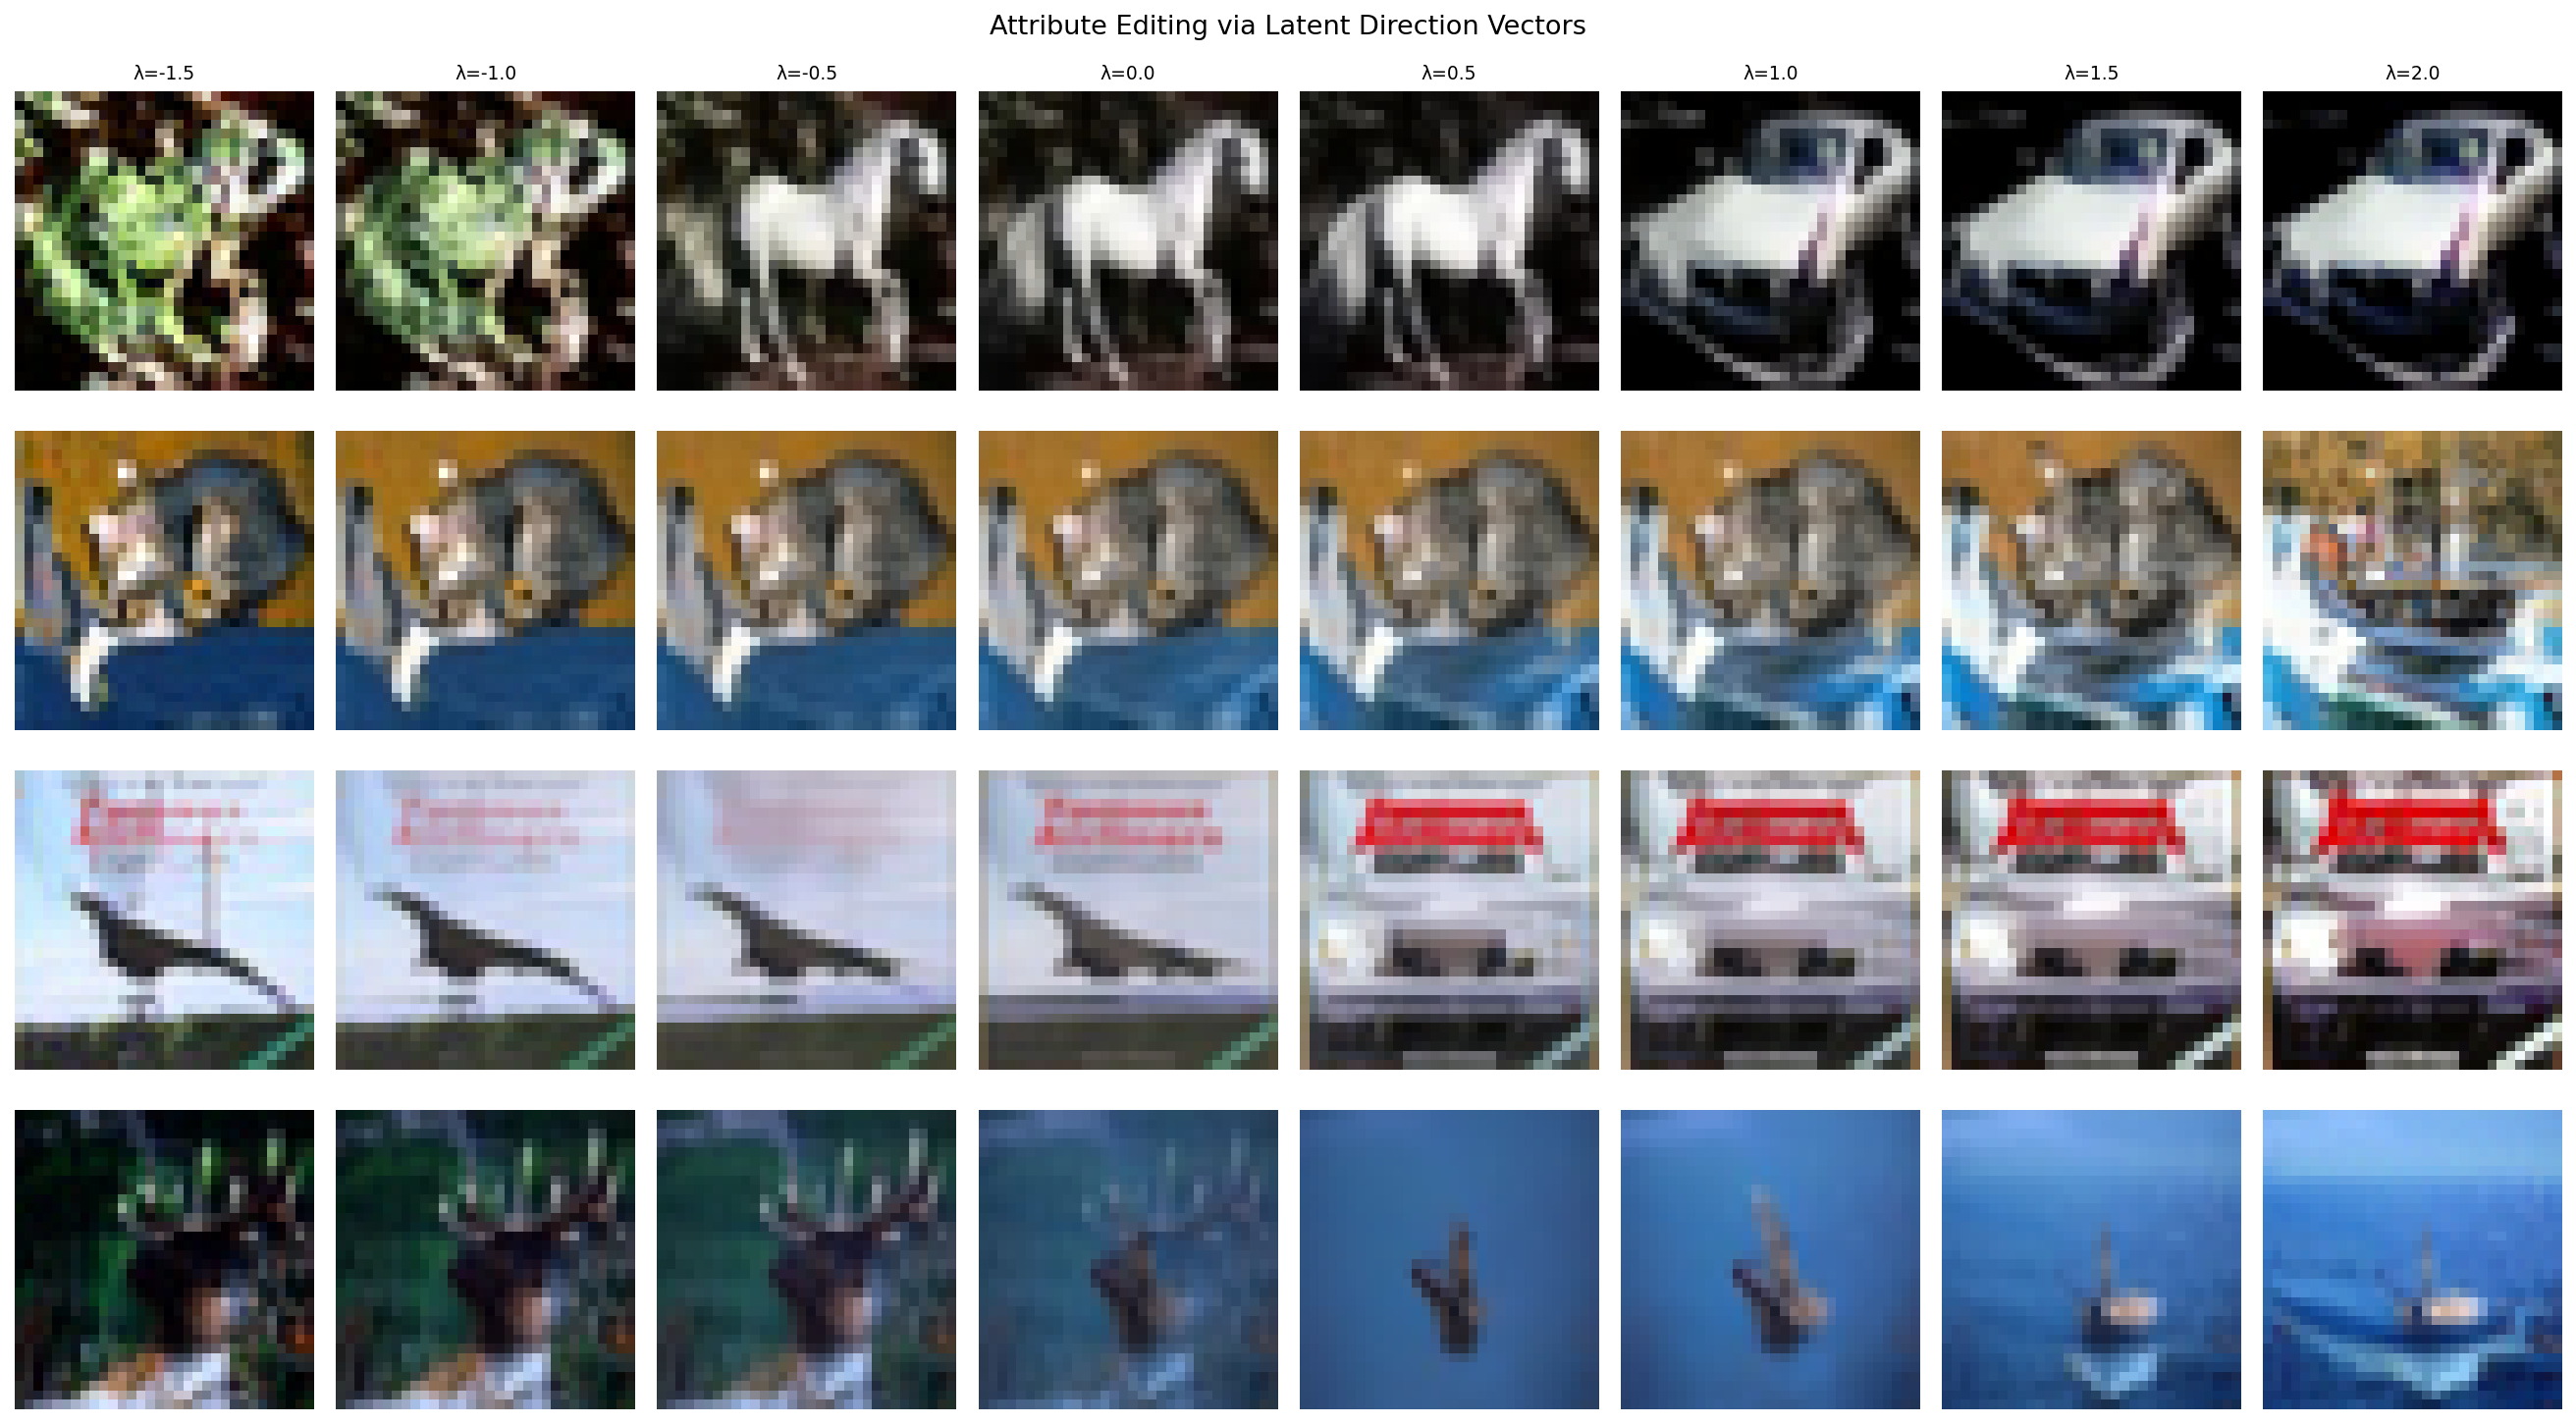
\includegraphics[width=\textwidth]{attribute_editing.png}\\[0.3em]
{\scriptsize $z_0^{\text{edit}} = z_0 + \lambda(\bar{z}_0^{\text{tgt}} - \bar{z}_0^{\text{src}})$\\
$\lambda{=}0$: original. $\lambda{>}0$: toward target.\\
e.g.\ horse$\to$car, cat$\to$dog.\\
Subtle but directional at 32$\times$32.}
\end{column}
\end{columns}
\end{frame}

\begin{frame}{Real image interpolation}
\centering
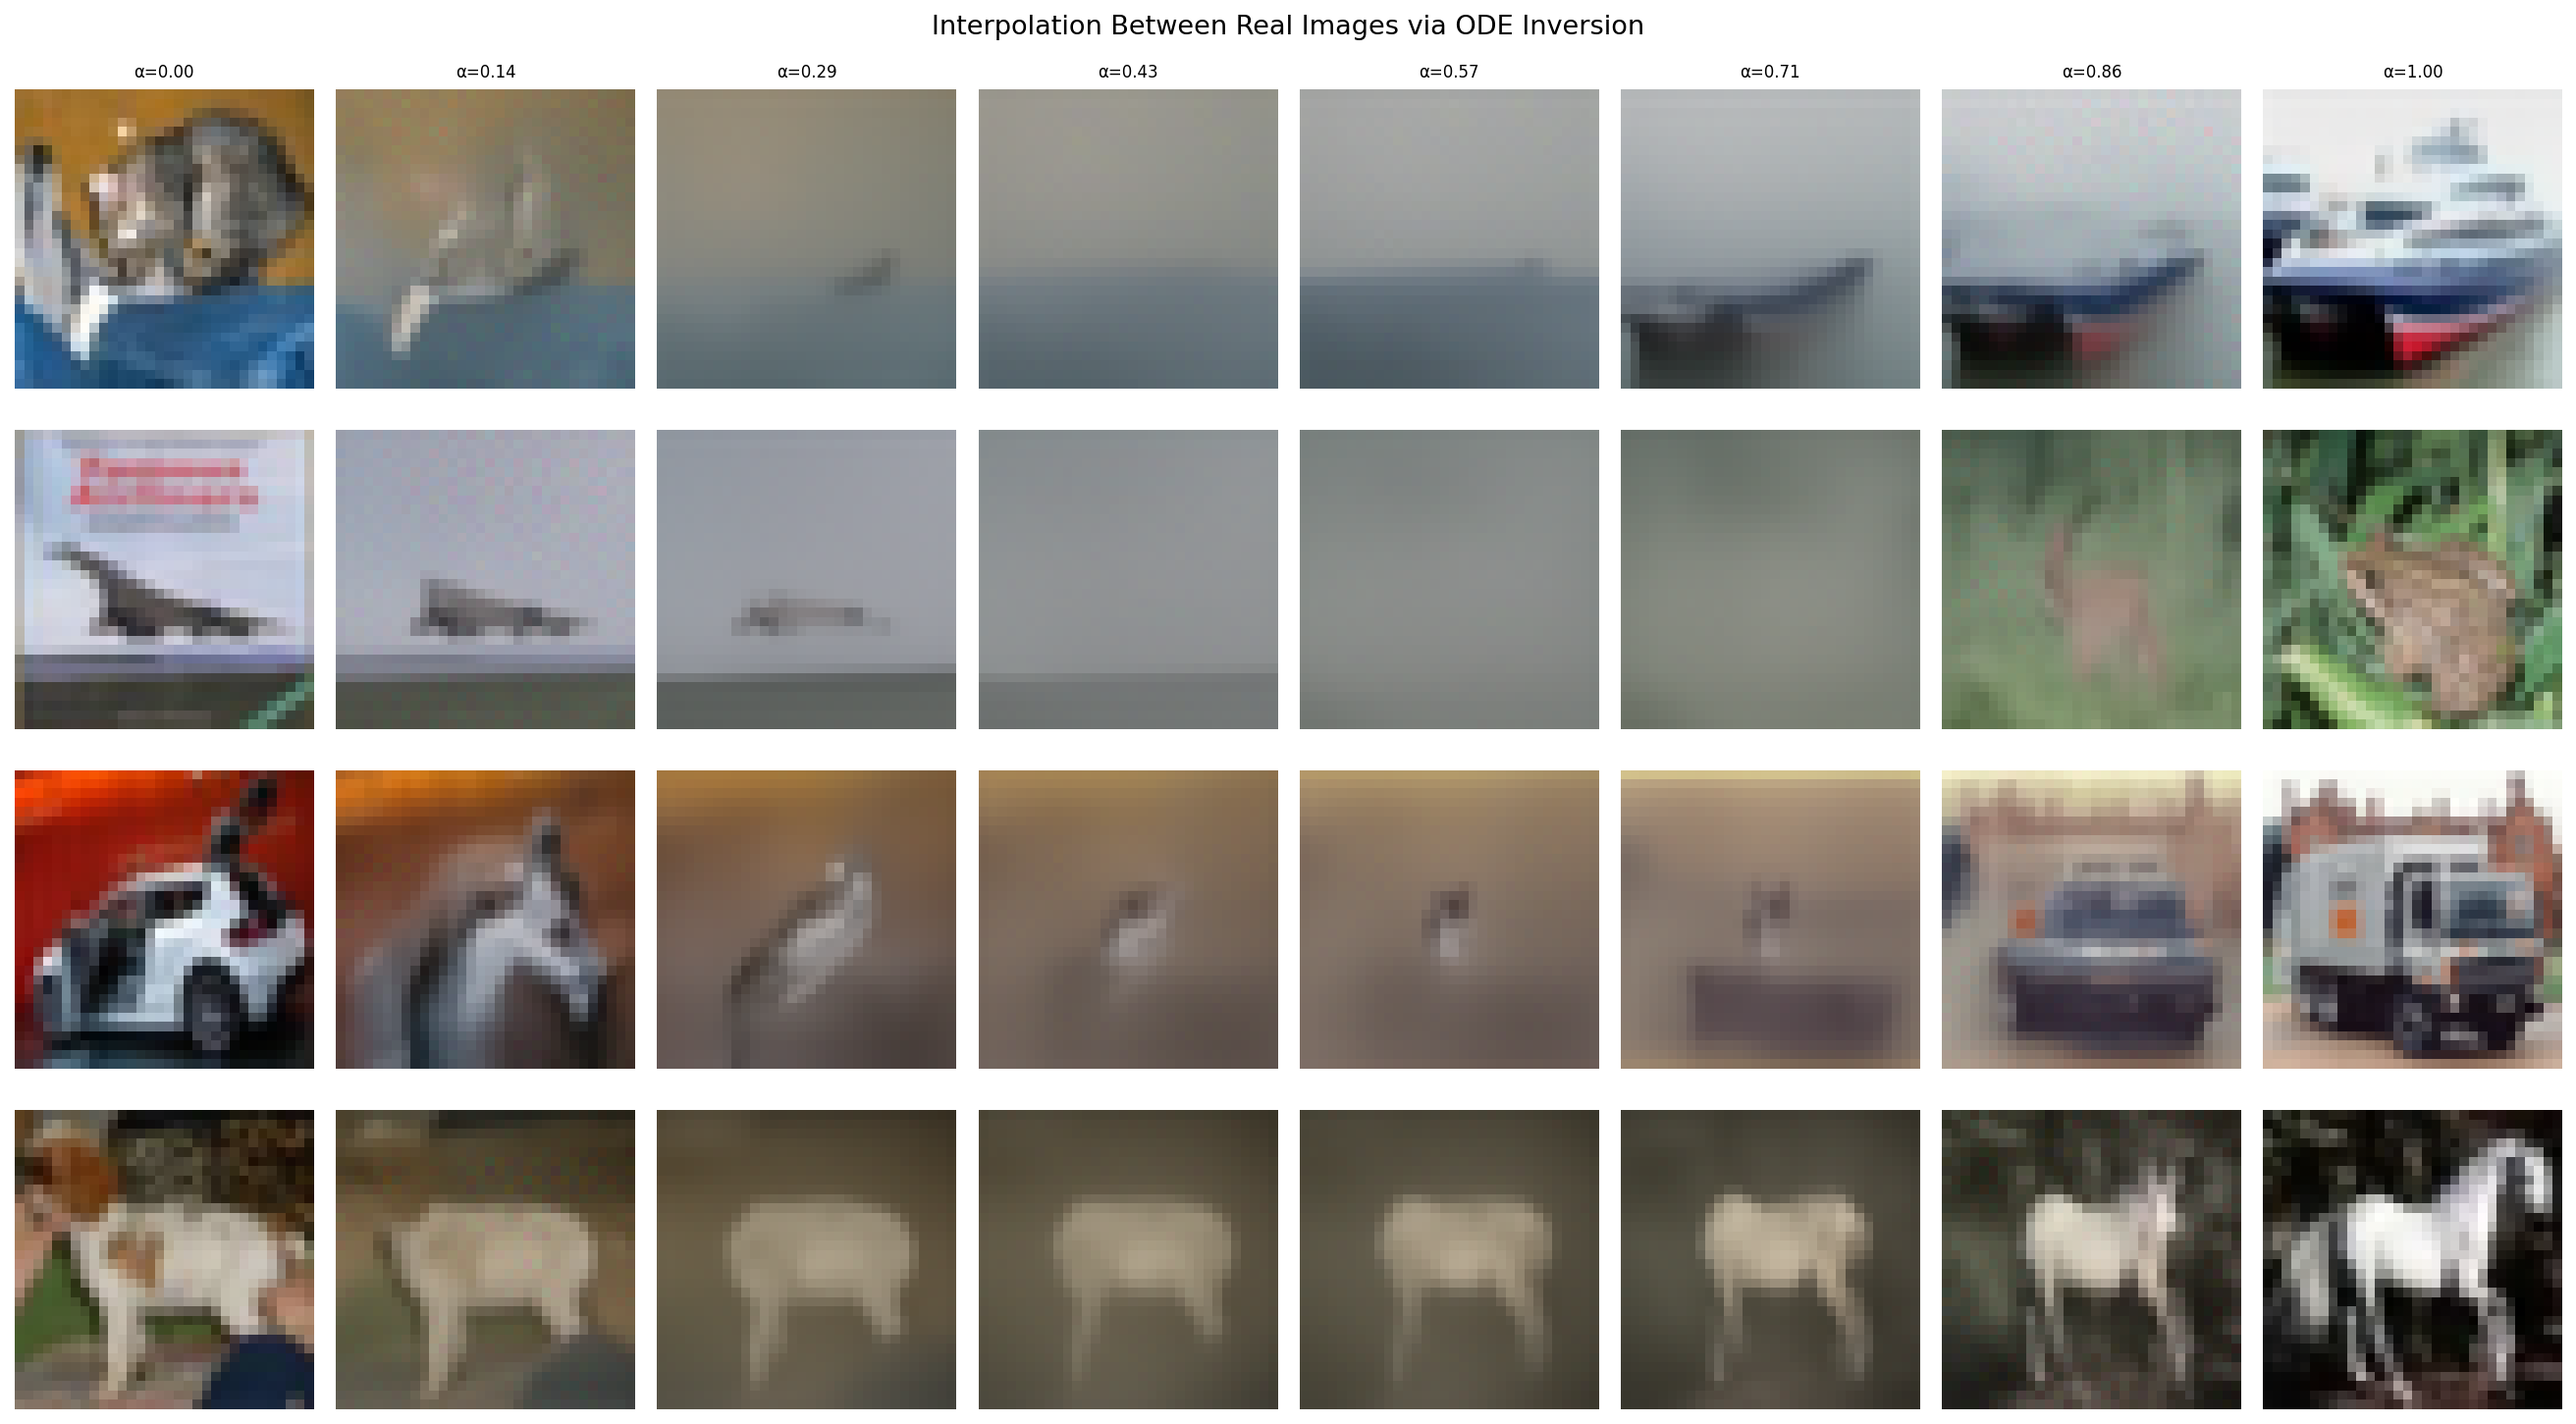
\includegraphics[width=0.85\textwidth]{real_interpolation.png}

\vspace{0.5em}
Encode two real images $\to$ $z_0^A$, $z_0^B$, then decode blends:
$z_0^{\alpha} = (1{-}\alpha)\,z_0^A + \alpha\,z_0^B$

\vspace{0.3em}
Unlike random-noise interpolation, this guarantees \textbf{real images at both endpoints}.
Smooth, semantically meaningful transitions through latent space.
\end{frame}

% ============================================================
\section{Analysis}

\begin{frame}{Why does flow matching win?}
\begin{columns}[T]
\begin{column}{0.48\textwidth}
\textbf{\textcolor{ddpmred}{Diffusion (DDPM/DDIM)}}
\begin{itemize}
    \item Learns noise prediction $\epsilon_\theta$
    \item Curved denoising paths
    \item DDIM: deterministic but approximate
    \item Quality saturates at $\sim$50 steps
    \item \alert{FID degrades past 50 NFE}
\end{itemize}
\end{column}
\begin{column}{0.48\textwidth}
\textbf{\textcolor{cfmblue}{Flow Matching (OT-CFM)}}
\begin{itemize}
    \item Learns velocity field $v_\theta$
    \item \textcolor{cfmblue}{Straight OT paths}
    \item Exact ODE formulation
    \item Quality \textcolor{accentgreen}{keeps improving} with NFE
    \item \textcolor{accentgreen}{Best at every NFE budget}
\end{itemize}
\end{column}
\end{columns}

\vspace{1em}
\centering
\textbf{Root cause}: OT-CFM's straight paths are easy for ODE solvers.\\
DDIM inherits errors from stochastic training $\Rightarrow$ error accumulation.
\end{frame}

\begin{frame}{Solver comparison \& DDIM saturation}
\begin{columns}[T]
\begin{column}{0.60\textwidth}
\centering

\begin{figure}
    \centering
    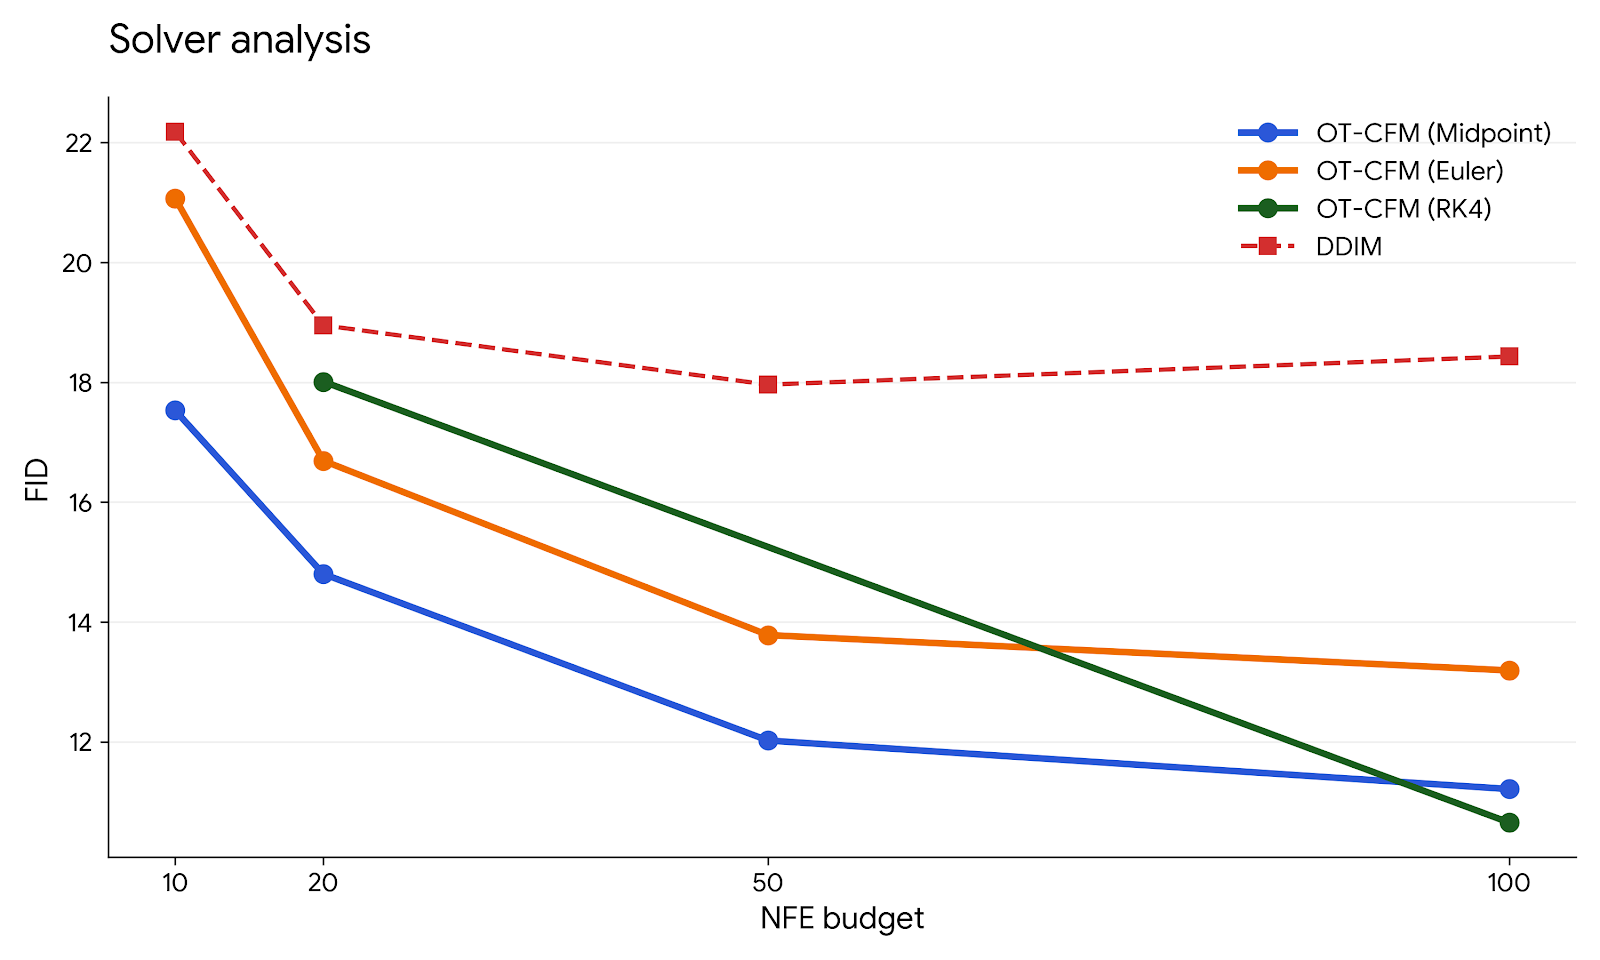
\includegraphics[width=1.05\linewidth]{comparaison_FID.png}
    \label{fig:placeholder}
\end{figure}
\end{column}
\begin{column}{0.45\textwidth}
\textbf{Solver choice:}
\begin{itemize}
    \item \textbf{Midpoint}: best at low NFE (10--50)
    \item \textbf{RK4}: best absolute FID at 100 NFE
    \item \textbf{Euler}: simplest, worst per-NFE
\end{itemize}

\vspace{0.5em}
\textbf{DDIM saturation:}
\begin{itemize}
    \item FID \alert{worsens} from 50$\to$100 NFE
    \item Stochastic training + deterministic sampling $\Rightarrow$ error accumulation
    \item CFM: no mismatch, FID \textcolor{accentgreen}{keeps improving}
\end{itemize}

\vspace{0.5em}
\textbf{Recommendation}: Midpoint for fast, RK4 for best quality.
\end{column}
\end{columns}
\end{frame}

% ============================================================
\section{Conclusion}

\begin{frame}{Key takeaways}
\begin{enumerate}
    \item \textbf{Flow matching $>$ diffusion} at every NFE budget on CIFAR-10
    \vspace{0.5em}
    \item \textbf{20$\times$ speedup}: OT-CFM matches DDPM quality in $\sim$50 steps vs.\ 1000
    \vspace{0.5em}
    \item \textbf{Best FID: 10.65} (OT-CFM + RK4 at 100 NFE)
    \vspace{0.5em}
    \item \textbf{Midpoint solver} recommended for low-NFE regimes
    \vspace{0.5em}
    \item \textbf{CFG improves class fidelity} while trading off diversity
    \vspace{0.5em}
    \item \textbf{ODE inversion} enables image editing, a unique advantage of flow matching
\end{enumerate}
\end{frame}

\begin{frame}{Limitations \& future work}
\textbf{Limitations:}
\begin{itemize}
    \item Single dataset: CIFAR-10 at $32 \times 32$
    \item No confidence intervals (single runs)
    \item Conditional model undertrained (210 vs.\ 500 epochs)
\end{itemize}

\vspace{1em}
\textbf{Future directions:}
\begin{itemize}
    \item Scale to higher resolutions (64$\times$64, 256$\times$256)
    \item Explore $\sigma_{\min}$ and advanced OT solvers
    \item Adaptive step-size ODE solvers
    \item Combine with latent diffusion / VAE framework
\end{itemize}
\end{frame}

\begin{frame}{What each of us did}
\begin{columns}[T]
\begin{column}{0.48\textwidth}
\textbf{\textcolor{cfmblue}{Ali Dor}}
\begin{itemize}
    \item DDPM / DDIM implementation
    \item ODE inversion \& image editing
    \item Visualizations:
    \begin{itemize}
        \item 2D toy experiments
        \item Generation trajectories
        \item Latent interpolations
    \end{itemize}
    \item Systematic NFE/solver evaluation
    \item Results analysis
\end{itemize}
\end{column}
\begin{column}{0.48\textwidth}
\textbf{\textcolor{accentgreen}{Elora Drouilhet}}
\begin{itemize}
    \item OT-CFM implementation
    \item Class-conditional CFM
    \begin{itemize}
        \item Class embeddings
        \item Classifier-free guidance
    \end{itemize}
    \item Model training \& evaluation
    \item CFG scale analysis
    \item Results analysis
\end{itemize}
\end{column}
\end{columns}
\end{frame}

\begin{frame}[plain]
\centering
\vfill
{\Huge\bfseries Thank you!}\\[1.5em]
{\large Questions?}\\[2em]
{\small Ali Dor \& Elora Drouilhet}\\
{\small CentraleSup\'elec}
\vfill
\end{frame}

\begin{frame}{References}
\footnotesize
\begin{thebibliography}{9}

\bibitem{lipman2023flow}
Y.~Lipman et al.
\newblock Flow matching for generative modeling.
\newblock In \emph{ICLR}, 2023.

\bibitem{tong2024improving}
A.~Tong et al.
\newblock Improving and generalizing flow-based generative models with minibatch optimal transport.
\newblock \emph{TMLR}, 2024.

\bibitem{ho2020denoising}
J.~Ho et al.
\newblock Denoising diffusion probabilistic models.
\newblock In \emph{NeurIPS}, 2020.

\bibitem{song2021denoising}
J.~Song et al.
\newblock Denoising diffusion implicit models.
\newblock In \emph{ICLR}, 2021.

\end{thebibliography}
\end{frame}

\end{document}
